\clearpage
\section{Optimizing Segment Length}\label{SegmentLength_MCBNBRecoTrack_section}
This section describes the study conducted to optimize the segment length in the algorithm. The input sample for this study was the high statistics simulated BNB neutrino interactions without any cosmics simulated described in Section \ref{MCBNB_input_sample_section}, and this study uses reconstructed tracks that have been selected according to the cuts described in Section \ref{MCBNBRecoTrack_eventselection_section}.\\

One of the tunable parameters in the MCS algorithm is the length of segments into which a track is divided. While shorter segment lengths yield more segments per track and therefore more sampling points to build a stronger likelihood, they also lead to the breakdown of the gaussian nature of scatters. Longer segments tend to have a more gaussian distribution of scatters but lead to fewer sampling points and therefore worse momentum resolution. For these reasons there exists an optimal segment length. Figure \ref{Highland_seglenstudy_MCBNBRecoTracks_fig} shows analogous figures to Figure \ref{Highland_validation_MCBNBRecoTrack_fig} for four different segment lengths ranging between 5 cm and 20 cm, with the same input sample of tracks. From this figure it can be seen that only segment lengths longer than or equal to 10 cm provide reasonably gaussian distributions.\\
Figure \ref{seglenstudy_bias_resolution_MCBNBRecoTrack_fig} shows the bias and resolution for the MCS momentum reconstruction method on this same sample. Here we see that shorter segment lengths tend to have a higher bias. Similarly, shorter segment lengths tend to have better resolution but the difference is small at larger momenta. For momenta below about 0.5 GeV the difference in resolution between segment lengths grows because the tracks are short enough that the longer segment lengths are not providing enough sampling points for the MCS method to make an accurate estimation of the track momentum. In order to maintain a gaussian distribution of angular scatters while providing enough sampling points for an momentum resolution of below 10\% for the shortest viable tracks, a segment length of 14 cm has been chosen for this analysis.

\begin{figure}
\centering
\mbox{
	\subfigure[\textit{Highland validation figure for 5 cm segment lengths.}]
	{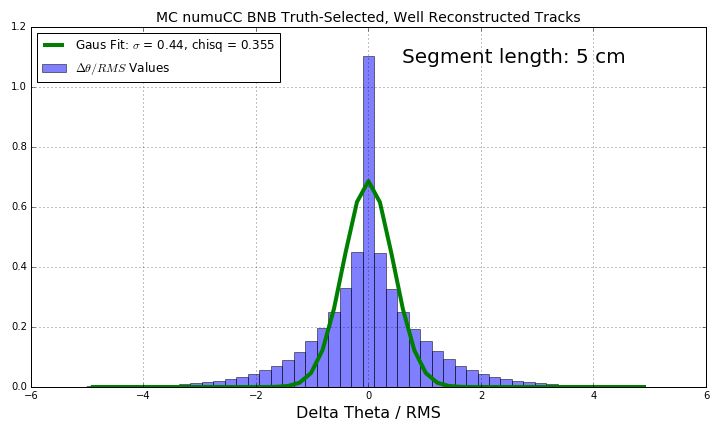
\includegraphics[width=75mm]{Figures/seglenstudy_gaus_5cm.png}}
	\quad
	\subfigure[\textit{Highland validation figure for 10 cm segment lengths.}]
	{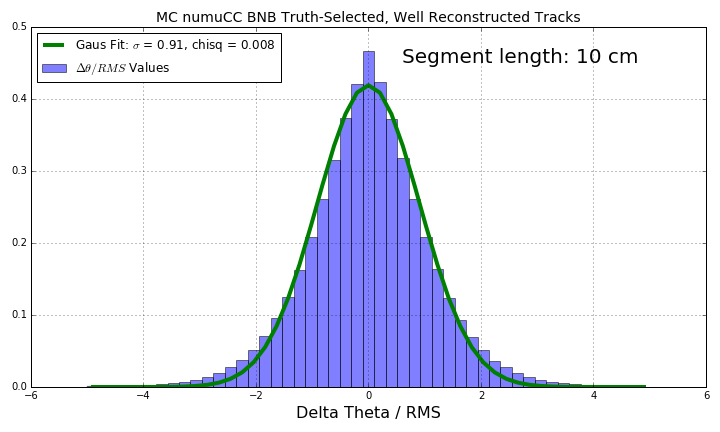
\includegraphics[width=75mm]{Figures/seglenstudy_gaus_10cm.png}}
	}\newline
\mbox{
	\subfigure[\textit{Highland validation figure for 14 cm segment lengths.}]
	{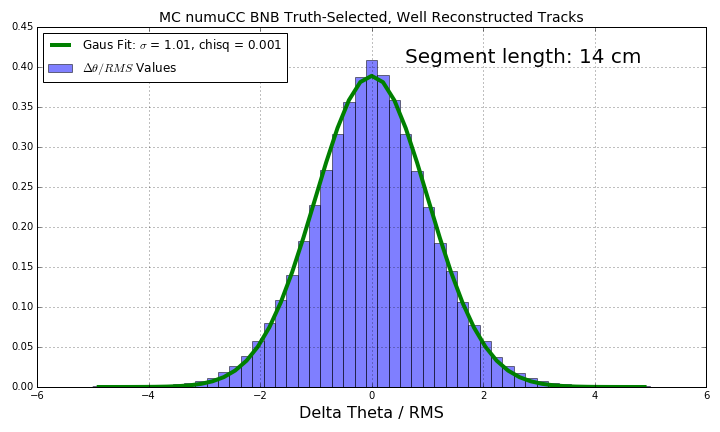
\includegraphics[width=75mm]{Figures/seglenstudy_gaus_14cm.png}}
	\quad
	\subfigure[\textit{Highland validation figure for 20 cm segment lengths.}]
	{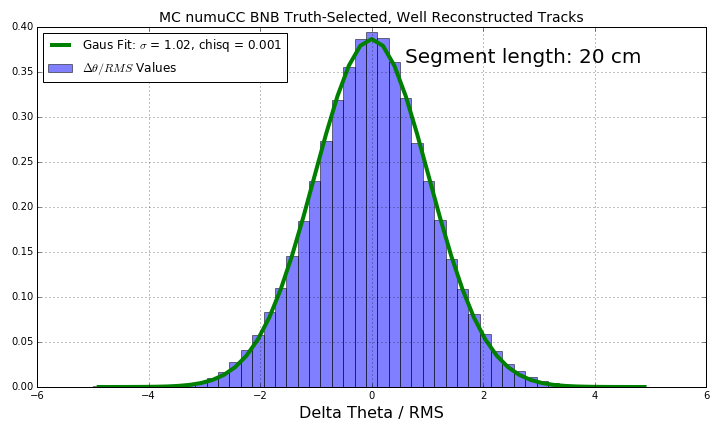
\includegraphics[width=75mm]{Figures/seglenstudy_gaus_20cm.png}}
	}
\caption{\textit{Highland validation figures analogous to Figure \ref{Highland_validation_MCBNBRecoTrack_fig} for various segment lengths, taken from the sample of well reconstructed neutrino-induced truth-selected muons in simulation. The gaussian nature of this plot breaks down for segment lengths that are too short.}}
\label{Highland_seglenstudy_MCBNBRecoTracks_fig}
\end{figure}



\begin{figure}
\centering
\mbox{
	\subfigure[\textit{MCS momentum bias as a function of range momentum for six different segment lengths. The vertical error bars are computed as $\frac{\sigma_{fit}}{\sqrt{N}}$, and the horizontal error bars indicate bin width.}]
	{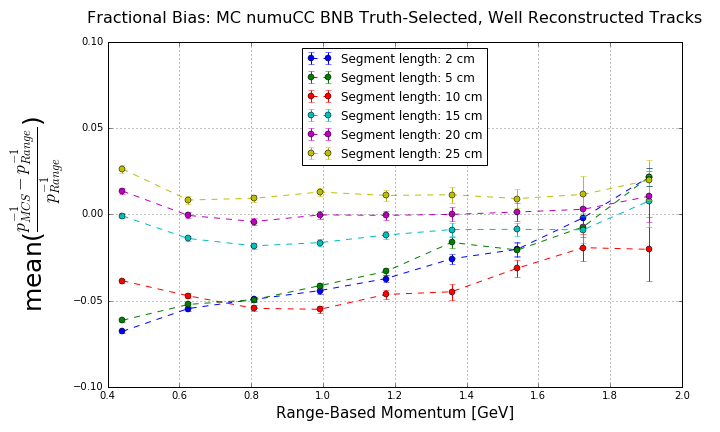
\includegraphics[width=75mm]{Figures/seglenstudy_MCBNBRecoTrack_bias.png}}
	\quad
	\subfigure[\textit{MCS momentum resolution as a function of range momentum for six different segment lengths. The vertical error bars are computed as $\frac{\sigma_{fit}}{\sqrt{2N}}$, and the horizontal error bars indicate bin width.}]
	{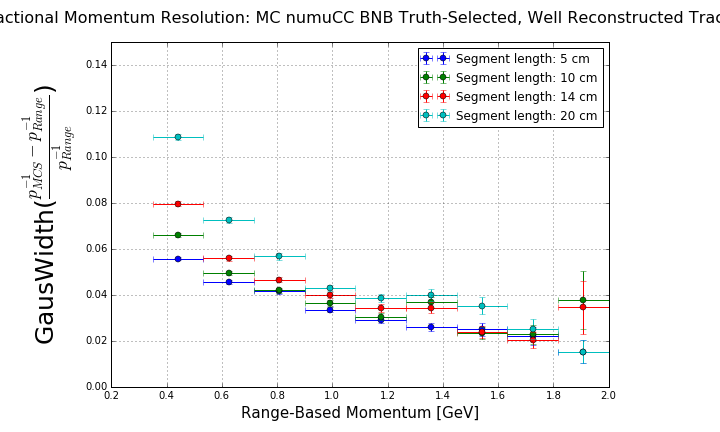
\includegraphics[width=75mm]{Figures/seglenstudy_MCBNBRecoTrack_resolution.png}}
	}
\caption{\textit{MCS momentum bias and resolution as a function of range momentum for the selected, well reconstructed neutrino-induced truth-selected muons in simulation.}}
\label{seglenstudy_bias_resolution_MCBNBRecoTrack_fig}
\end{figure}





















\clearpage
\section{Optimizing Constant Detector Resolution Term}\label{ResolutionStudy_MCBNBRecoTrack_section}
This section describes how the resolution term $\sigma_o^{res}$ in the modified Highland equation, Equation \ref{modified_highland_eqtn} is chosen. The input sample for this study was the high statistics simulated BNB neutrino interactions without any cosmics simulated described in Section \ref{ExitingStudy_MCBNBRecoTrack_section}, and this study uses exiting reconstructed tracks that have been selected according to the cuts described in that section. The reason that exiting tracks are used is that the detector-inherent resolution term only begins to become relevant at muon momenta above the maximum possible for contained tracks in the TPC, as for lower momentum the physical scatters are larger than the resolution term. A muon traversing the entire director would be roughly 10 meters long, which corresponds to a total momentum of around 2.3 GeV, which corresponds to an RMS scattering angle predicted $\sigma_o$ of 5 mrad at the start of the track if 14 cm segments are used (as seen in Figure \ref{retune_highland_fig4}). This resolution constant was chosen \textit{after} choosing the optimal segment length of 14 cm described in Appendix \ref{SegmentLength_MCBNBRecoTrack_section}. In order to choose a resolution term, a procedure similar to the one described in the segment length optimization section (Appendix \ref{SegmentLength_MCBNBRecoTrack_section}) is followed. This sample of well-reconstructed truth-selected exiting muons from numu charged current interactions in simulation was analyzed with various different resolution terms.\\

The momentum bias and resolution are computed in the usual way for different resolution terms, using the nominal 14 cm segment length in the algorithm. The results can be seen in Figures \ref{ResolutionStudy_MCBNBRecoTrackExiting_bias_fig} and \ref{ResolutionStudy_MCBNBRecoTrackExiting_resolution_fig} respectively. While the resolution isn't very sensitive to the choice of resolution term, the bias is. Looking at the 0 mrad resolution points (blue) in the bias figure, one can see the bias increases starting around 2 GeV. This is because above this momentum, the angular scatters are small enough to be comparable with the detector-inherent angular resolution. To account for this, the resolution term is slowly increased, flattening out the bias. It was found that a resolution of 3 mrad (the cyan points) makes the bias the most flat across all momenta. Note that a resolution term greater than 3 mrad actually causes the bias to go negative at higher momenta. For this reason, 3 mrad is chosen as the optimal detector-inherent angular resolution term, $\sigma_o$ in Equation \ref{modified_highland_eqtn} for all analyses based on reconstructed tracks. Note that for analyses based on {\sc MCTracks}, $\sigma_o$ is set to zero because {\sc MCTracks} have perfect resolution.

\begin{figure}
\centering
\mbox{
	\subfigure[\textit{MCS momentum bias as a function of true momentum for four different resolution terms. The vertical error bars are computed as $\frac{\sigma_{fit}}{\sqrt{N}}$, and the horizontal error bars indicate bin width.}\label{ResolutionStudy_MCBNBRecoTrackExiting_bias_fig} ]
	{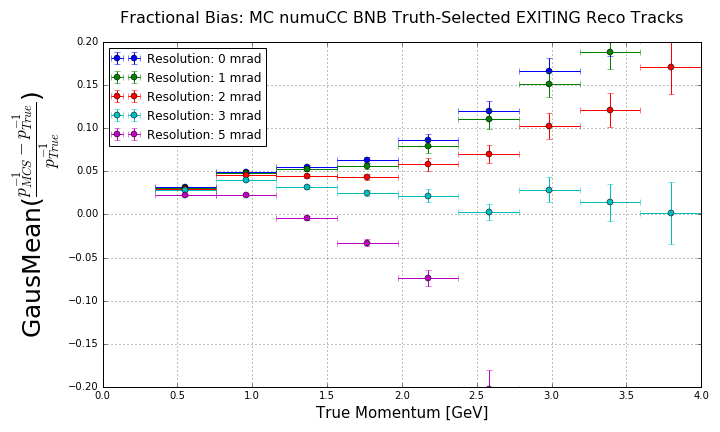
\includegraphics[width=75mm]{Figures/resstudy_MCBNBRecoTrackExiting_bias.png}}
	\quad
	\subfigure[\textit{MCS momentum resolution as a function of true momentum for four different resolution terms. The vertical error bars are computed as $\frac{\sigma_{fit}}{\sqrt{2N}}$, and the horizontal error bars indicate bin width.}\label{ResolutionStudy_MCBNBRecoTrackExiting_resolution_fig} ]
	{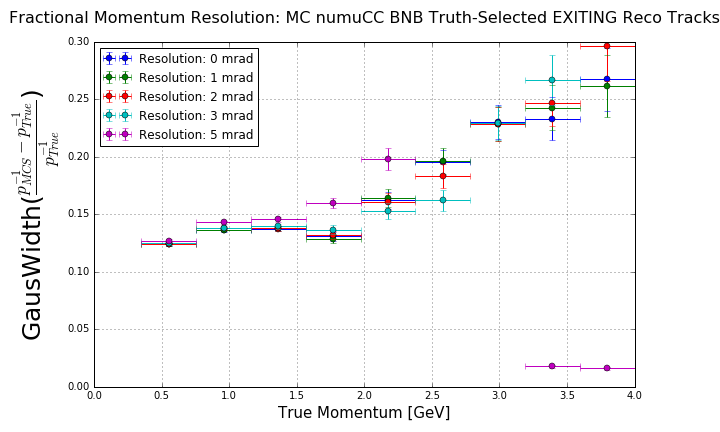
\includegraphics[width=75mm]{Figures/resstudy_MCBNBRecoTrackExiting_resolution.png}}
	}
\caption{\textit{The impact of constant resolution terms, $\sigma_o^{res}$ in the modified Highland equation, Equation \ref{modified_highland_eqtn}, on exiting reconstructed tracks.}}
\end{figure}





















\clearpage
\section{MCS to Determine Track Direction}\label{TrackDirection_MCBNBRecoTrack_section}
This section demonstrates the ability for the multiple coulomb scattering algorithm to determine the direction of a (fully contained) track. The input sample for this study was the high statistics simulated BNB neutrino interactions without any cosmics simulated described in Section \ref{MCBNB_input_sample_section}, and this study uses reconstructed tracks that have been selected according to the cuts described in Section \ref{MCBNBRecoTrack_eventselection_section}. The MCS code as it is described in Section \ref{MCS_technique_section} works by maximizing a likelihood based on angular scatters between segments of a track along with the expected RMS angular deviation from the modified Highland equation (Equation \ref{modified_highland_eqtn}). In practice, there is actually a negative log likelihood that is minimized, meaning the lower the likelihood the more confident the fit is. In order to determine the direction of a track with MCS, one can compute the converged minimum negative log likelihood for the track assuming it is oriented in the correct direction, then reverse the ordering of the trajectory points in the track and compute the converged minimum negative log likelihood for the reversed track. The likelihood should be better (smaller) for tracks in the correct direction than their reversed counterparts.\\

Given this truth-selected sample in simulation, the true direction of the track is known. The minimized negative log likelihood for each of these tracks both in the correct (forwards) direction and incorrect (backwards) direction can be seen in Figure \ref{TrackDirection_MCBNBRecoTrack_LLHDoverlay_fig}. A smaller likelihood here means a better fit in the MCS code. Figure \ref{TrackDirection_MCBNBRecoTrack_LLHDdiff_fig} shows the track-by-track difference of these two distributions, forwards minus backwards. Any negative entries in this figure indicate that the forwards-going track had a better fit than backwards-going. This figure shows that MCS can be a powerful tool to test track direction.

\begin{figure}
\centering
\mbox{
	\subfigure[\textit{The minimized negative log likelihood value for each track in the well-reconstructed, fully contained neutrino-induced truth-selected muon tracks in simulation sample, both with tracks oriented in the correct (forwards) direction and reversed (backwards) direction. A smaller likelihood here means a better fit in the MCS code.}\label{TrackDirection_MCBNBRecoTrack_LLHDoverlay_fig}]
	{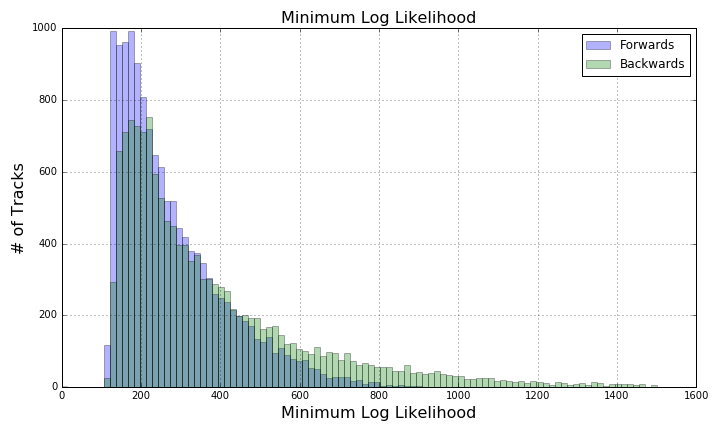
\includegraphics[width=75mm]{Figures/TrackDirection_MCBNBRecoTrack_LLHDoverlay.png}}
	\quad
	\subfigure[\textit{The track-by-track difference, forwards minus backwards, of the log likelihoods. Negative entries indicate that the forwards-going tracks had a better fit than the backwards-going ones.}\label{TrackDirection_MCBNBRecoTrack_LLHDdiff_fig}]
	{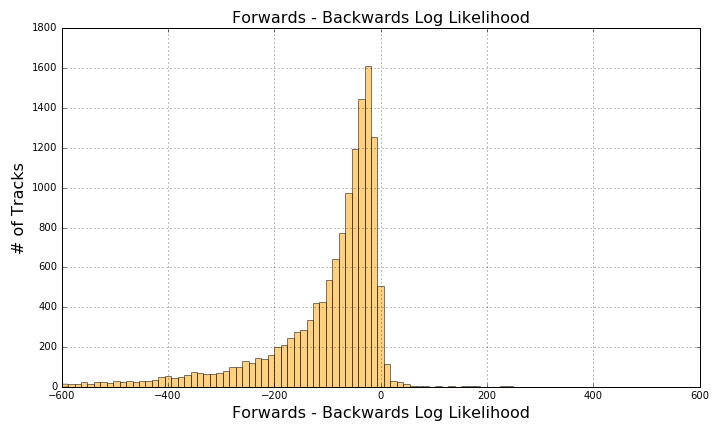
\includegraphics[width=75mm]{Figures/TrackDirection_MCBNBRecoTrack_LLHDdiff.png}}
	}
\caption{\textit{Evidence that MCS can be used to determine track directions by analyzing the output of the likelihood fit.}}
\end{figure}




















\clearpage
\section{Inverse Momentum to Quantify Resolution: Justification}\label{inverse_p_justification_section}
Throughout this note, the bias and resolution for the MCS momentum estimation method have been computed by fitting gaussians to distributions of ($\frac{p_{MCS}^{-1} - p_{range}^{-1}}{p_{range}^{-1}}$). The Highland formula (Equation \ref{highland_eqtn}) predicts gaussian-distributed angular scatters $\Delta\theta$ and is a function of $\frac{1}{p}$. As described by the Opera paper on multiple coulomb scattering\cite{OPERA_paper}, ``since the inverted momentum distribution $\frac{1}{p}$ has a Gaussian shape, the width of the Gaussian divided by $\frac{1}{p_{mean}}$ directly gives the momentum resolution estimate $\frac{\Delta(1/p)}{(1/p)}.$''

Purely for visualization sake, to demonstrate that distributions of ($\frac{p_{MCS}^{-1} - p_{range}^{-1}}{p_{range}^{-1}}$) are more gaussian than distributions of ($\frac{p_{MCS} - p_{range}}{p_{range}}$), Figure \ref{MCS_gausvalidation_twoslices_fig} shows each of these distributions for reconstructed tracks with range energy between 0.35 and 0.53 GeV from the sample of the high statistics simulated BNB neutrino interactions without any cosmics simulated described in Section \ref{MCBNB_input_sample_section}.\\

\begin{figure}
\centering
\mbox{
	\subfigure[\textit{Fractional momentum difference using inverse momentum, including gaussian fit.}]
	{\includegraphics[width=75mm]{Figures/{MCS_range_resolution_MCBNBRecoTrack_GAUSVALIDATION_inverse_gaus_slice_0.35_0.53}.png}}
	\quad
	\subfigure[\textit{Fractional momentum difference using normal momentum, including gaussian fit.}]
	{\includegraphics[width=75mm]{Figures/{MCS_range_resolution_MCBNBRecoTrack_GAUSVALIDATION_normal_gaus_slice_0.35_0.53}.png}}
}
\caption{\textit{Fractional momentum differences between 0.35 and 0.53 GeV range energy for well reconstructed muons from the simulated BNB sample with truth-based selection.}}
\label{MCS_gausvalidation_twoslices_fig}
\end{figure}


% Throughout this note, the bias and resolution for the MCS momentum estimation method have been computed by fitting gaussians to distributions of ($\frac{p_{MCS}^{-1} - p_{range}^{-1}}{p_{range}^{-1}}$). Note that this is algebraically equivalent to ($\frac{p_{range} - p_{MCS}}{p_{MCS}}$). The reason that the inverse momentum is used is that these distributions are more gaussian, and therefore fitting a gaussian to them and using the result of that (the mean for the bias and the width for the resolution) is more appropriate. In this section, several ways of computing the bias and resolution are demonstrated:
% \begin{enumerate}
% 	\item Fitting gaussians to distributions of ($\frac{p_{MCS}^{-1} - p_{range}^{-1}}{p_{range}^{-1}}$) and using the resulting fit $\sigma$ and $\mu$ for resolution and bias estimates (respectively).
% 	\item Fitting gaussians to distributions of ($\frac{p_{MCS} - p_{range}}{p_{range}}$) and using the resulting fit $\sigma$ and $\mu$ for resolution and bias estimates (respectively).
% 	\item Simply using the standard deviation and mean of ($\frac{p_{MCS}^{-1} - p_{range}^{-1}}{p_{range}^{-1}}$) to estimate the resolution and the bias (respectively).
% 	\item Simply using the standard deviation and mean of ($\frac{p_{MCS} - p_{range}}{p_{range}}$) to estimate the resolution and the bias (respectively).
% \end{enumerate}
% The differences between these methods are described and the choice of using option (1) throughout the note is justified.\\



% The input sample for this study was the high statistics simulated BNB neutrino interactions without any cosmics simulated described in Section \ref{MCBNB_input_sample_section}, and this study uses reconstructed tracks that have been selected according to the cuts described in Section \ref{MCBNBRecoTrack_eventselection_section}.\\

% To demonstrate that distributions of ($\frac{p_{MCS}^{-1} - p_{range}^{-1}}{p_{range}^{-1}}$) are more gaussian than distributions of ($\frac{p_{MCS} - p_{range}}{p_{range}}$), Figure \ref{MCS_gausvalidation_twoslices_fig} shows each of these distributions for reconstructed tracks with range energy between 0.35 and 0.53 GeV. This slice was chosen because it has the highest statistics.\\

% \begin{figure}
% \centering
% \mbox{
% 	\subfigure[\textit{Fractional momentum difference using inverse momentum, including gaussian fit.}]
% 	{\includegraphics[width=75mm]{Figures/{MCS_range_resolution_MCBNBRecoTrack_GAUSVALIDATION_inverse_gaus_slice_0.35_0.53}.png}}
% 	\quad
% 	\subfigure[\textit{Fractional momentum difference using normal momentum, including gaussian fit.}]
% 	{\includegraphics[width=75mm]{Figures/{MCS_range_resolution_MCBNBRecoTrack_GAUSVALIDATION_normal_gaus_slice_0.35_0.53}.png}}
% }

% \caption{\textit{Fractional momentum differences between 0.35 and 0.53 GeV range energy for well reconstructed muons from the simulated BNB sample with truth-based selection.}}
% \label{MCS_gausvalidation_twoslices_fig}
% \end{figure}

% Figures \ref{MCS_gausvalidation_bias_fig} and \ref{MCS_gausvalidation_resolution_fig} show the bias and resolution as a function of range for the four different methods of computing outlined above. In general, all four methods result in similar bias and resolutions, however the resolution when using standard devition of normal momentum (option 4) is slightly worse. \textbf{It can be seen that when using inverse momentum, the bias and resolutions computed with gaussian fits agree well with those computed from mean and std of underlying distributions (Figures \ref{MCS_gausvalidation_bias_fig}(a) and (c) agree better than Figures \ref{MCS_gausvalidation_bias_fig}(b) and (d), and Figures \ref{MCS_gausvalidation_resolution_fig}(a) and (c) agree better than Figures \ref{MCS_gausvalidation_resolution_fig}(b) and (d)). This serves as motivation to use inverse momentum rather than normal momentum.}

% \begin{figure}
% \centering
% \mbox{
% 	\subfigure[\textit{Bias computed with gaussian fits to inverse momentum.}]
% 	{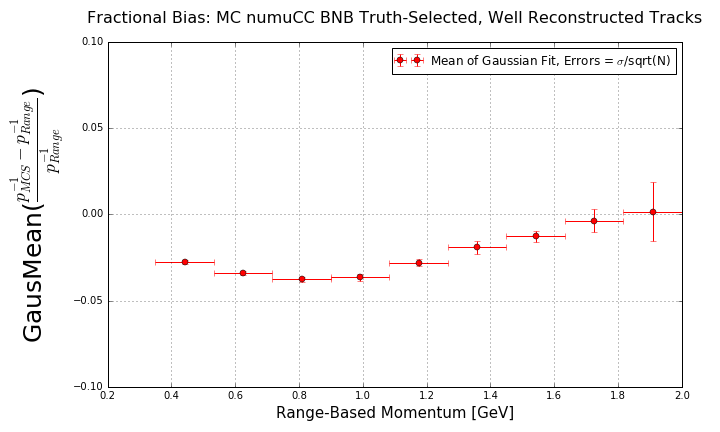
\includegraphics[width=75mm]{Figures/MCS_range_bias_MCBNBRecoTrack_GAUSVALIDATION_inverse_gaus.png}}
% 	\quad
% 	\subfigure[\textit{Bias computed with gaussian fits to normal momentum.}]
% 	{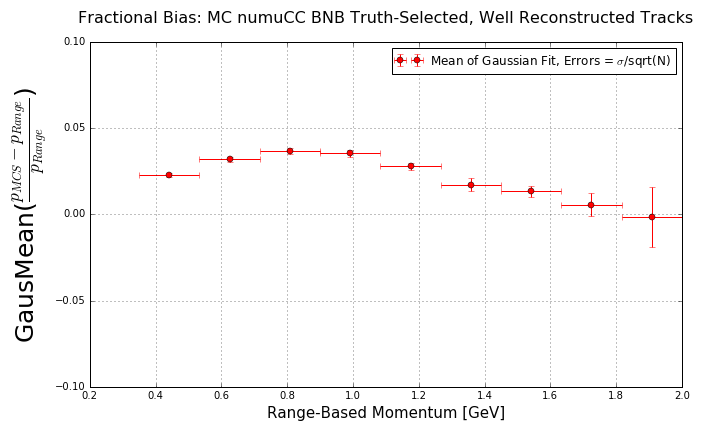
\includegraphics[width=75mm]{Figures/MCS_range_bias_MCBNBRecoTrack_GAUSVALIDATION_normal_gaus.png}}
% }

% \mbox{
% 	\subfigure[\textit{Bias computed with mean of inverse momentum distributions.}]
% 	{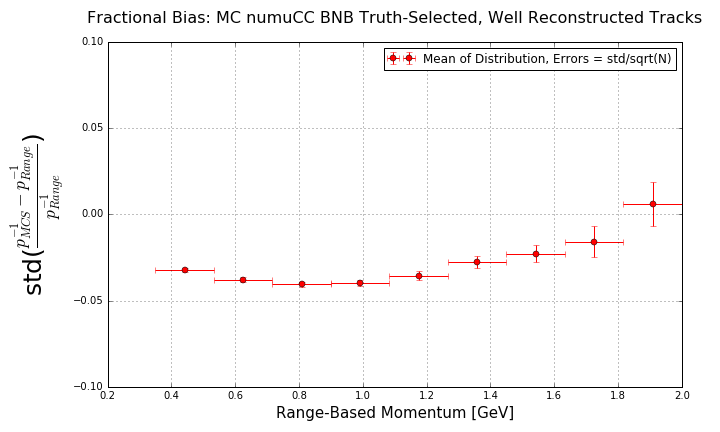
\includegraphics[width=75mm]{Figures/MCS_range_bias_MCBNBRecoTrack_GAUSVALIDATION_inverse_std.png}}
% 	\quad
% 	\subfigure[\textit{Bias computed with mean of normal momentum distributions.}]
% 	{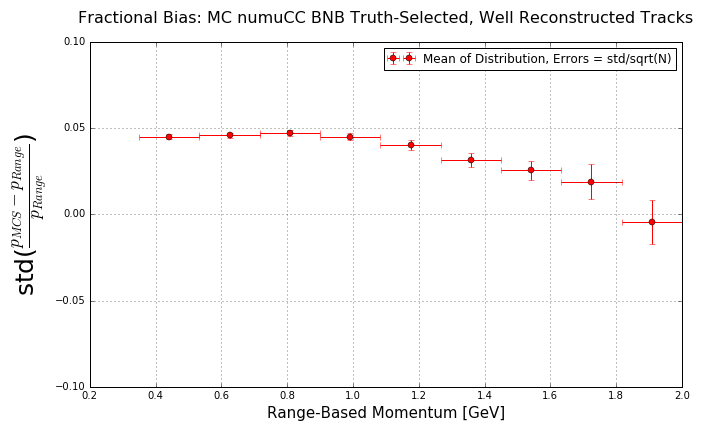
\includegraphics[width=75mm]{Figures/MCS_range_bias_MCBNBRecoTrack_GAUSVALIDATION_normal_std.png}}
% }
	
% \caption{\textit{MCS bias as a function of range energy computed four different ways for well reconstructed muons from the simulated BNB sample with truth-based selection.}}
% \label{MCS_gausvalidation_bias_fig}
% \end{figure}

% \begin{figure}
% \centering
% \mbox{
% 	\subfigure[\textit{Resolution computed with gaussian fits to inverse momentum.}]
% 	{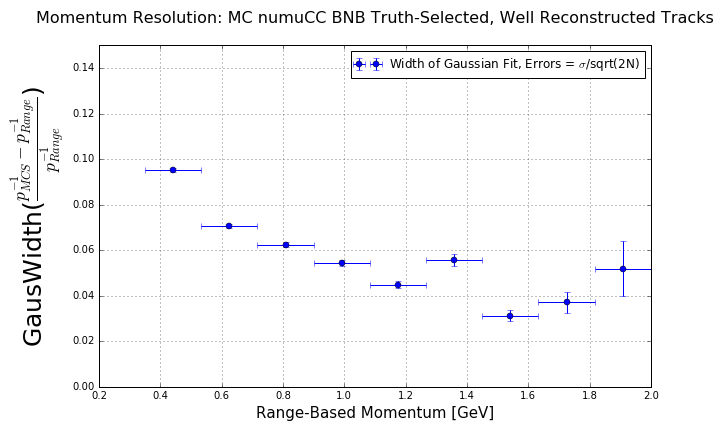
\includegraphics[width=75mm]{Figures/MCS_range_resolution_MCBNBRecoTrack_GAUSVALIDATION_inverse_gaus.png}}
% 	\quad
% 	\subfigure[\textit{Resolution computed with gaussian fits to normal momentum.}]
% 	{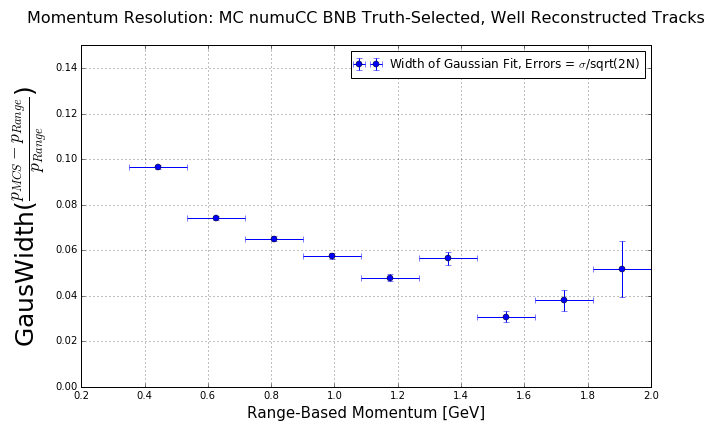
\includegraphics[width=75mm]{Figures/MCS_range_resolution_MCBNBRecoTrack_GAUSVALIDATION_normal_gaus.png}}
% }

% \mbox{
% 	\subfigure[\textit{Resolution computed with std of inverse momentum distributions.}]
% 	{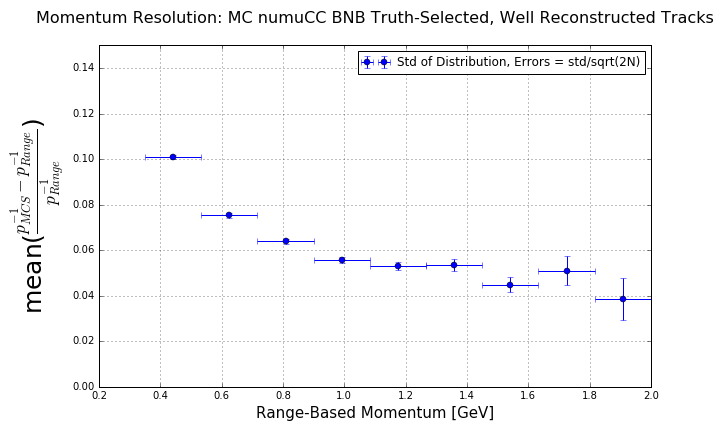
\includegraphics[width=75mm]{Figures/MCS_range_resolution_MCBNBRecoTrack_GAUSVALIDATION_inverse_std.png}}
% 	\quad
% 	\subfigure[\textit{Resolution computed with std of normal momentum distributions.}]
% 	{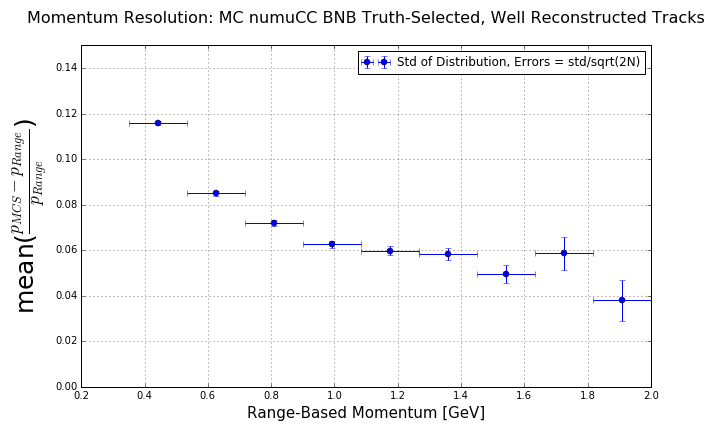
\includegraphics[width=75mm]{Figures/MCS_range_resolution_MCBNBRecoTrack_GAUSVALIDATION_normal_std.png}}
% }
	
% \caption{\textit{MCS resolution as a function of range energy computed four different ways for well reconstructed muons from the simulated BNB sample with truth-based selection.}}
% \label{MCS_gausvalidation_resolution_fig}
% \end{figure}




















\clearpage
\section{Track Angle Dependence}\label{AngleStudy_MCBNBRecoTrack_section}
This section describes a brief study of how the performance of the MCS algorithm varies with track angle. The angles of interest are both with respect to the drift direction $x-$, and with respect to the vertical (collection plane wire orientation) direction $y-$. The input sample for this study was the high statistics simulated BNB neutrino interactions without any cosmics simulated described in Section \ref{MCBNB_input_sample_section}, and this study uses reconstructed tracks that have been selected according to the cuts described in Section \ref{MCBNBRecoTrack_eventselection_section}.\\

The usual bias and resolution plots as a function of range-based momentum for four different bins of angle with respect to the drift direction are shown in Figure \ref{xangle_bias_resolution_fig}. Despite limited statistics, it is clear that there is only minimal performance change as a function of angle with respect to the drift direction.\\

The usual bias and resolution plots as a function of range-based momentum for four different bins of angle with respect to the vertical (collection wire plane orientation) direction are shown in Figure \ref{yangle_bias_resolution_fig}. Despite limited statistics, it is clear that there is only minimal performance change as a function of angle with respect to the vertical direction.\\



\begin{figure}
\centering
\mbox{
	\subfigure[\textit{MCS momentum bias as a function of range-based momentum. The vertical error bars are computed as $\frac{\sigma_{fit}}{\sqrt{N}}$, and the horizontal error bars indicate bin width.}]
	{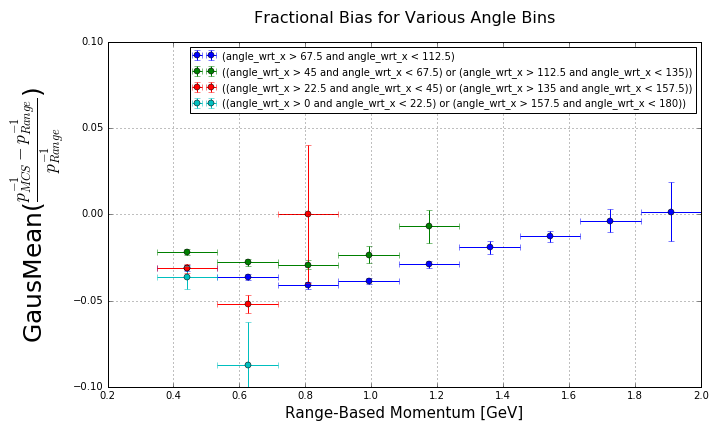
\includegraphics[width=75mm]{Figures/MCS_range_bias_anglestudy_xangle.png}}
	\quad
	\subfigure[\textit{MCS momentum resolution as a function of range-based momentum. The vertical error bars are computed as $\frac{\sigma_{fit}}{\sqrt{2N}}$, and the horizontal error bars indicate bin width.}]
	{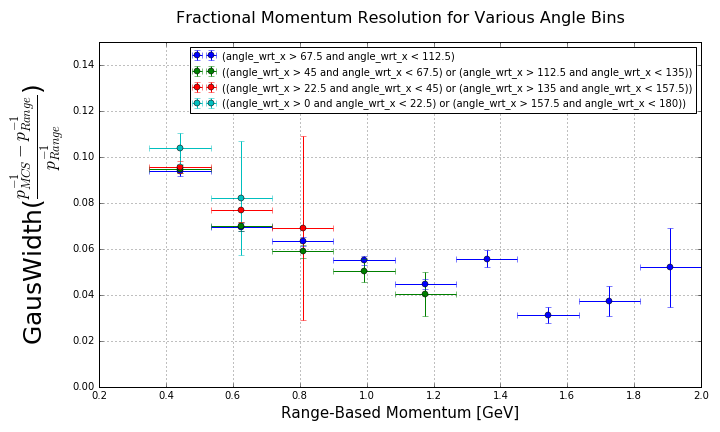
\includegraphics[width=75mm]{Figures/MCS_range_resolution_anglestudy_xangle.png}}
	}
\caption{\textit{MCS momentum bias and resolution as a function of range momentum for the truth-selected simulated fully contained, well reconstructed muon tracks from numu charged current events. Resolution is broken into four bins of angle with respect to the drift direction: blue are tracks perpendicular to the drift direction to within 22.5 degrees, and cyan are tracks oriented parallel to the drift direction to within 22.5 degrees.}}
\label{xangle_bias_resolution_fig}
\end{figure}


\begin{figure}
\centering
\mbox{
	\subfigure[\textit{MCS momentum bias as a function of range-based momentum. The vertical error bars are computed as $\frac{\sigma_{fit}}{\sqrt{N}}$, and the horizontal error bars indicate bin width.}]
	{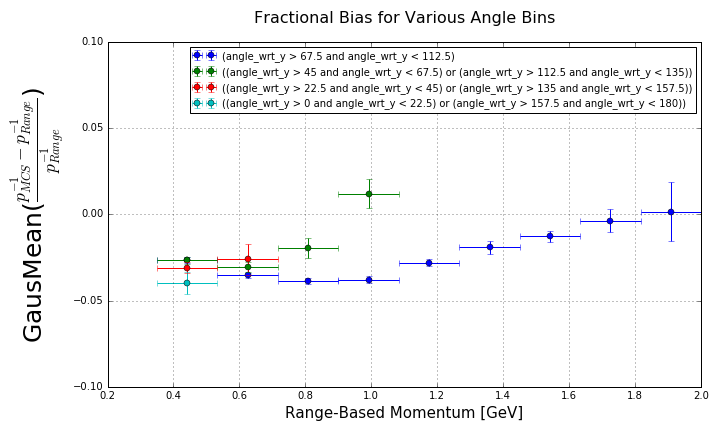
\includegraphics[width=75mm]{Figures/MCS_range_bias_anglestudy_yangle.png}}
	\quad
	\subfigure[\textit{MCS momentum resolution as a function of range-based momentum. The vertical error bars are computed as $\frac{\sigma_{fit}}{\sqrt{2N}}$, and the horizontal error bars indicate bin width.}]
	{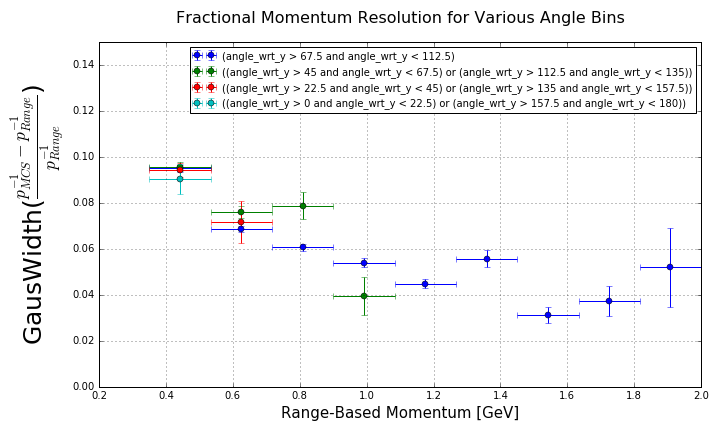
\includegraphics[width=75mm]{Figures/MCS_range_resolution_anglestudy_yangle.png}}
	}
\caption{\textit{MCS momentum bias and resolution as a function of range momentum for the truth-selected simulated fully contained, well reconstructed muon tracks from numu charged current events. Resolution is broken into four bins of angle with respect to the vertical (collection plane wire orientation) direction: blue are tracks perpendicular to the vertical direction to within 22.5 degrees, and cyan are tracks oriented parallel to the vertical direction to within 22.5 degrees.}}
\label{yangle_bias_resolution_fig}
\end{figure}























\clearpage
\section{Effect of Removing the End of Tracks}\label{CutStudy_MCBNBRecoTrack_section}
This section describes a brief study of how the performance of the MCS algorithm changes when the ends of tracks are removed. Note that the reader can refer to studies of \textit{exiting} tracks elsewhere in this note for an additional handle on how algorithm performance changes when the ends of tracks are not visible (for example Section \ref{ExitingStudy_MCBNBRecoTrack_section}).\\


The input sample for this study was the high statistics simulated BNB neutrino interactions without any cosmics simulated described in Section \ref{MCBNB_input_sample_section}, and this study uses fully contained reconstructed tracks that have been selected according to the cuts described in Section \ref{MCBNBRecoTrack_eventselection_section}. This study is relevant for two reasons. First, removing the end of a track in a way simulates exiting tracks. Secondly, since the MCS algorithm takes into account energy loss in its likelihood (Section \ref{maximum_likelihood_section}), it is possible the algorithm is biased for fully contained tracks since it is cutting off postulated MCS energies which are less than the full track MIP energy loss. Removing the last many centimeters of a track helps prevent the cutting of these tails.\\

The usual bias and resolution plots as a function of true momentum for six different lengths of track cut are shown in Figure \ref{custudy_bias_resolution_fig}. It can be seen that the resolution worsens the more is removed from the end of the track. This intuitively makes sense because removing more track amounts to fewer measurements used to build the likelihood. It can also be seen that the fractional bias does \textit{not} improve when the end of the track is removed, indivating that the aforementioned cutting of low energy MCS tails is not a source of bias in the algorithm. When the last 4 segments (56 cm) of a track are removed, the resolution in the lowest energy bin (tracks approximately 1 meter in length) worsens from 8\% to about 20\%. For longer tracks the impact of removing the last 4 segments is much smaller, only worsening the resolution by a few percent. The algorithm bias is largely unaffected by the removal of the end of the track.\\

\begin{figure}
\centering
\mbox{
	\subfigure[\textit{MCS momentum bias as a function of true momentum. The vertical error bars are computed as $\frac{\sigma_{fit}}{\sqrt{N}}$, and the horizontal error bars indicate bin width.}]
	{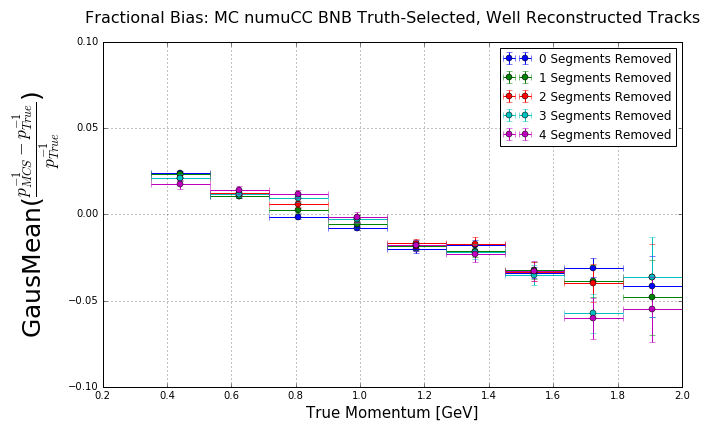
\includegraphics[width=75mm]{Figures/cutstudy_MCBNBRecoTrack_bias.png}}
	\quad
	\subfigure[\textit{MCS momentum resolution as a function of true momentum. The vertical error bars are computed as $\frac{\sigma_{fit}}{\sqrt{2N}}$, and the horizontal error bars indicate bin width.}]
	{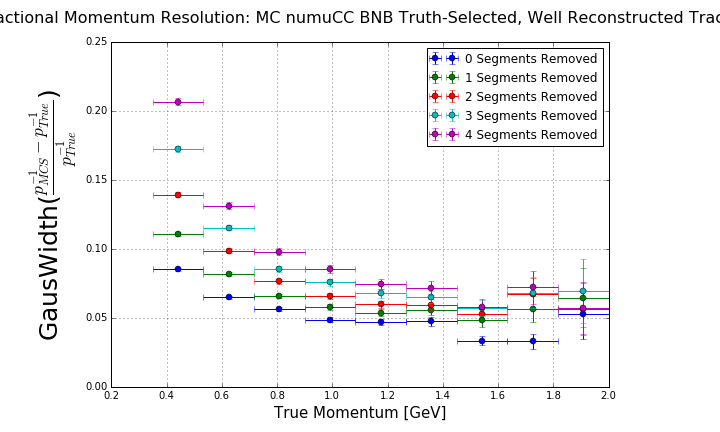
\includegraphics[width=75mm]{Figures/cutstudy_MCBNBRecoTrack_resolution.png}}
	}
\caption{\textit{MCS momentum bias and resolution as a function of true momentum for the truth-selected simulated fully contained, well reconstructed muon tracks from numu charged current events. Segment lengths are 14 cm, and the number of segments removed from the end of the track are shown in the legend.}}
\label{custudy_bias_resolution_fig}
\end{figure}
